\newpage
\section{Specifica del Back-End}
\subsection{QuizziPedia::Back-End}
\subsubsection{Informazioni generali}
\label{QuizziPedia::Back-End}
\begin{figure}
	\centering
	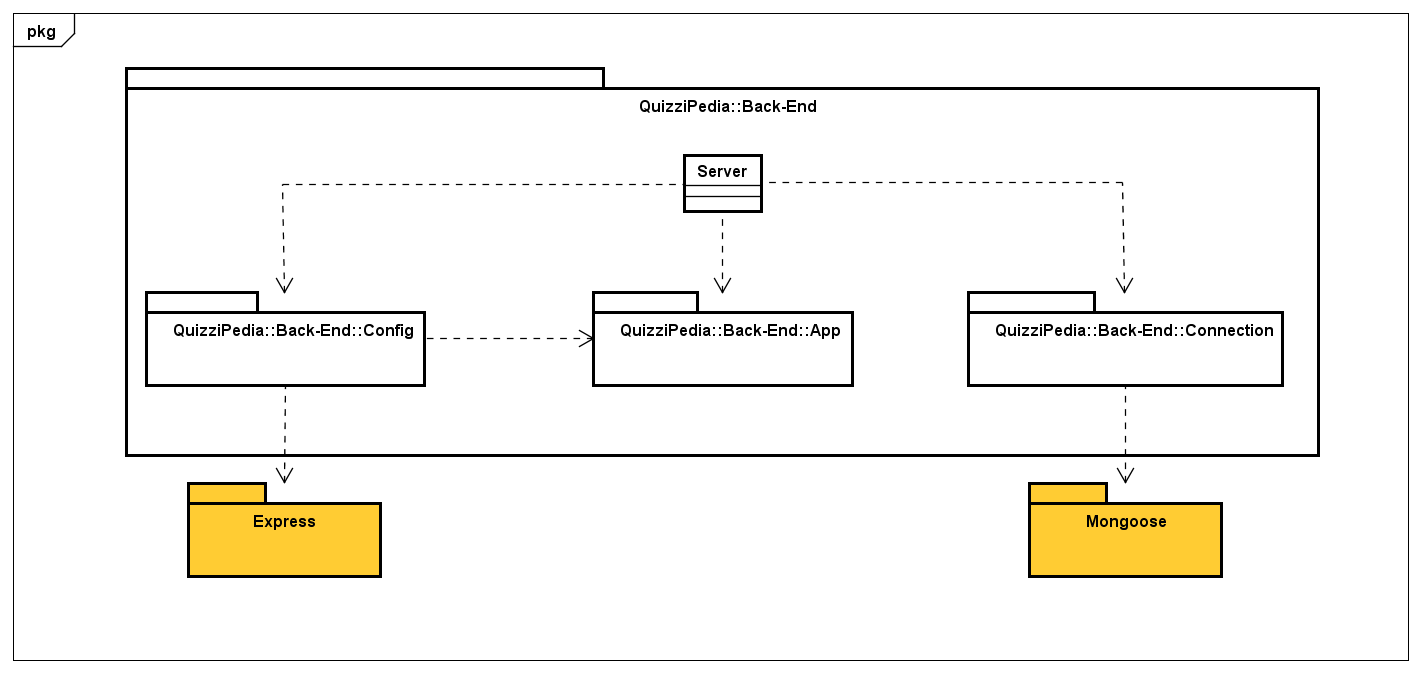
\includegraphics[scale=0.45]{UML/Package/QuizziPedia_Back-End.png}
	\caption{QuizziPedia::Back-End}
\end{figure}

	\begin{itemize}
		\item \textbf{Descrizione} \\ Package contenenti le componenti della parte back-end dell' applicazione.
		\item \textbf{Package contenuti}
		\begin{itemize}
			\item App \\
			Package\ped{G} contenente le componenti del server che implementano il \textit{pattern MVC\ped{G}}.
			\item Config \\
			Package\ped{G} contenente le componenti di configurazione del server\ped{G}.
		\end{itemize}
	\end{itemize}
\subsubsection{Classi}
	\paragraph{QuizziPedia::Back-End::Server}
	\begin{itemize}
		\item \textbf{Descrizione} \\
		Classe che avvia il server. Nello specifico apre una connessione al database tramite Mongoose, invoca il middleware\ped{G} Express\ped{G} passando un riferimento al database MongoDB\ped{G} come parametro in modo  che possa configurarsi con esso, invoca il middleware\ped{G} Passport\ped{G} ed infine si mette in ascolto su una determinata porta. E' il componente client del design pattern \textit{Chain of responsibility\ped{G}}. Utilizza i moduli Mongoose\ped{G}, Express\ped{G}, Passport\ped{G}.
		\item \textbf{Utilizzo} \\
		Utilizzo per avviare l'applicazione lato server. Inizializza, internamente al back-end, la catena di gestione delle chiamate REST\ped{G} utilizzando le classi contenute nel package \texttt{Routers}
		\item \textbf{Relazioni con altre classi}
		\item \textbf{Attributi}
		\item \textbf{Metodi}
	\end{itemize}
	
\subsection{QuizziPedia::Back-End::Config}
\subsubsection{Informazioni generali}
\label{QuizziPedia::Back-End::Config}
\begin{figure}
	\centering<
	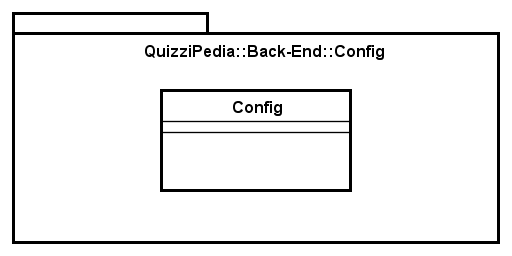
\includegraphics[scale=0.45]{UML/Package/QuizziPedia_Back-End_Config.png}
	\caption{QuizziPedia::Back-End::Config}
\end{figure}
	\begin{itemize}
		\item \textbf{Descrizione} \\
		Package contenente le copmonenti di configurazione del server.
		\item \textbf{Padre}: Back-End
		\item \textbf{Interazioni con altri componenti}:
			\begin{itemize}
				\item \texttt{App} \\
				Package contenente le componenti del server che implementano il \textit{pattern MVC\ped{G}}.
			\end{itemize}
	\end{itemize}
\subsubsection{Classi}
\paragraph{QuizziPedia::Back-End::Config::Config}
\label{QuizziPedia::Back-End::Config::Config}
\begin{figure}
	\centering
	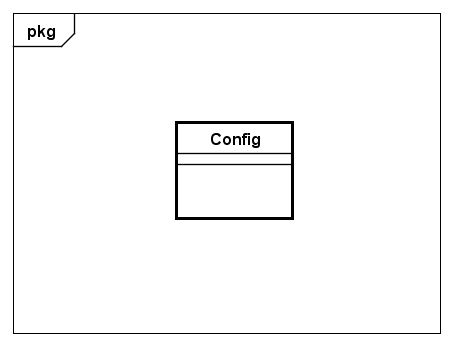
\includegraphics[scale=0.45]{UML/Package/QuizziPedia_Back-End_Config_Config.png}
	\caption{QuizziPedia::Back-End::Config::Config}
	\end{figure}
	\begin{itemize}
		\item \textbf{Descrizione} \\
		Questa classe gestisce la configurazione del server. \textit{Non sono stati modellati attributi e metodi di questa classe in quanto viene gestita da Express}
		\item \textbf{Utilizzo} \\
		Viene utilizzata per descrivere i parametri dell'applicazione. La classe \texttt{Server} utilizza oggetti di questo tipo per creare ed avviare l'istanza del server.
		\item \textbf{Relazioni con le altre classi}:
		 \begin{itemize}
		 	\item \textit{IN} \texttt{Server} \\
		 	Classe che avvia il server. Nello specifico apre una connessione al database tramite Mongoose, invoca il middleware\ped{G} Express\ped{G} passando un riferimento al database MongoDB\ped{G} come parametro in modo  che possa configurarsi con esso, invoca il middleware\ped{G} Passport\ped{G} ed infine si mette in ascolto su una determinata porta. E' il componente client del design pattern \textit{Chain of responsibility\ped{G}}. Utilizza i moduli Mongoose\ped{G}, Express\ped{G}, Passport\ped{G}.
		 \end{itemize}
	\end{itemize}


\subsection{QuizziPedia::Back-End::App}
\subsubsection{Informazioni generali}
\label{QuizziPedia::Back-End::App}
\begin{figure}
	\centering
	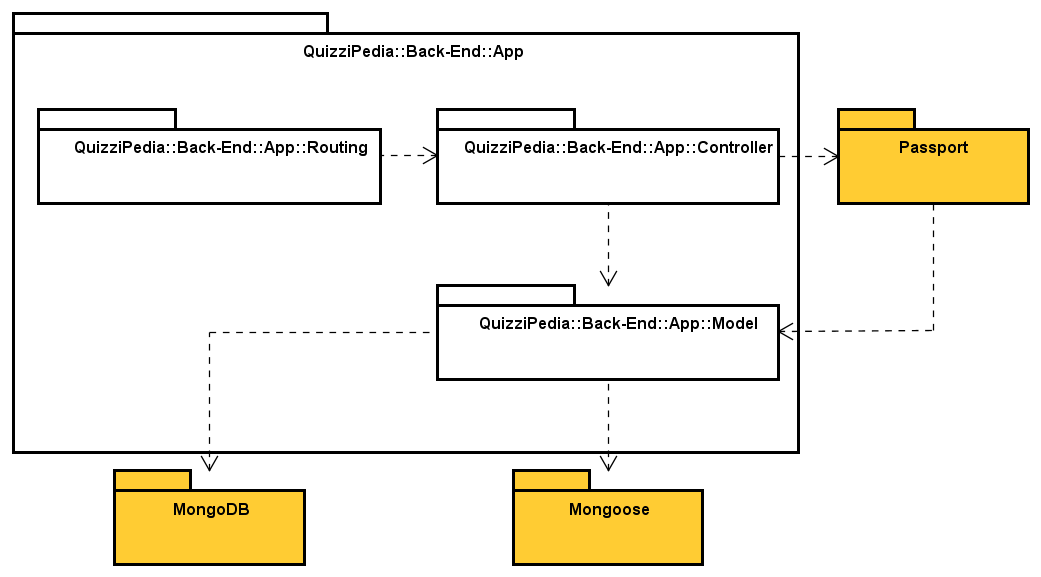
\includegraphics[scale=0.45]{UML/Package/QuizziPedia_Back-End_App.png}
	\caption{QuizziPedia::Back-End::App}
\end{figure}
	\begin{itemize}
		\item \textbf{Descrizione} \\
		Package contenente le componenti del server che implementano il \textit{pattern\ped{G} MVC\ped{G}};
		\item \textbf{Padre} \\ Back-End;
		\item \textbf{Interazioni con altri componenti}
			\begin{itemize}
				\item Congif \\
				Package contenente le componenti di configurazione del server;
			\end{itemize}
		\item \textbf{Package contenuti}
			\begin{itemize}
				\item Controllers \\
				Package che contiene i controllers di Express, definisce la logica dell'applicazione;
				\item Models \\
				Package che contiene le classi che definiscono il model dell'applicazione. Queste classi cono definite come classi schema di \textit{Mongoose\ped{G}}, il quale permette di utilizzare \textit{MongoDB\ped{G}} tramite degli oggetti;
				\item Routers \\
				Package contenente i routers della componente back-end dell'applicazione. Contiene i file di configurazione relativi al routing delle richieste del client, ossia i routers di Express.
			\end{itemize}
	\end{itemize}
	
\subsection{QuizziPedia::Back-End::App::Controllers}
\label{QuizziPedia::Back-End::App::Controllers}
\begin{figure}
	\centering
	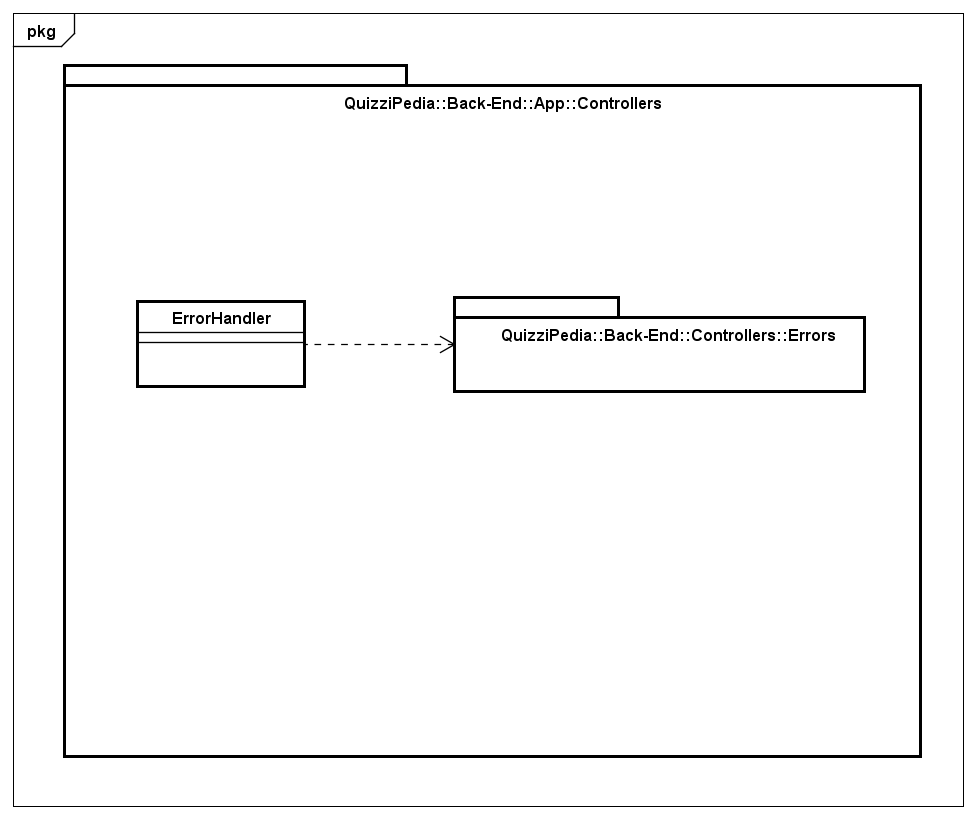
\includegraphics[scale=0.45]{UML/Package/QuizziPedia_Back-End_App_Controllers.png}
	\caption{QuizziPedia::Back-End::App::Controllers}
\end{figure}
\subsubsection{Informazioni generali}
	\begin{itemize}
		\item \textbf{Descrizione} \\
		Package contenente i controllers di Express, definisce la logica dell'applicazione.
		\item \textbf{Padre}: \texttt{App}
		\item \textbf{Interazioni con altri componenti}
			\begin{itemize}
				\item \texttt{Routers} \\
				Package contenente i router della componente back-end dell'applicazione. Contiene i file di configurazione relativi al routing delle richieste del client, ossia i routers di Express.
				\item \texttt{Views} \\
				Package contenente le views della copmonente back-end dell'applicazione.
			\end{itemize}
		\item \textbf{Package contenuti}:
			\begin{itemize}
				\item \texttt{Errors} \\
				Package contenente i controllers per la gestione degli errori specifici.
			\end{itemize}
	\end{itemize}
\subsubsection{Classi}
\paragraph{QuizziPedia::Back-End::App::Controllers::NOMECLASSE}
	\begin{itemize}
		\item \textbf{Descrizione} \\
		\item \textbf{Utilizzo} \\
		\item \textbf{Relazioni con altre classi} \\
		\item \textbf{Metodi} \\
	\end{itemize}
	
\subsection{QuizziPedia::Back-End::App::Controllers::Errors}
\subsubsection{Informazioni generali}
\label{QuizziPedia::Back-End::App::Controllers::Errors}
\begin{figure}
	\centering
	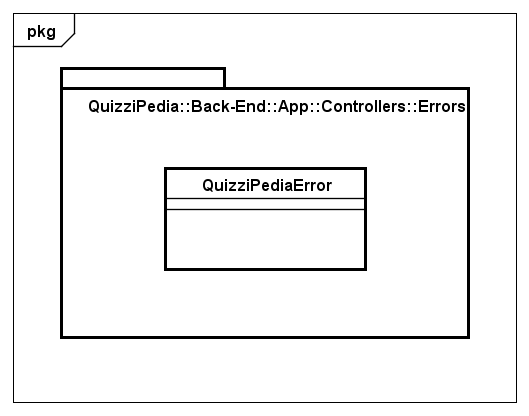
\includegraphics[scale=0.45]{UML/Package/QuizziPedia_Back-End_App_Controllers_Errors.png}
	\caption{QuizziPedia::Back-End::App::Controllers::Errors}
\end{figure}
	\begin{itemize}
		\item \textbf{Descrizione} \\
		Package contenente i controllers per la gestione degli errori specifici.
		\item \textbf{Padre}: \texttt{Controllers}
	\end{itemize}
\subsubsection{Classi}
\paragraph{QuizziPedia::Back-End::App::Controllers::Errors::QuizziPediaErrors}
	\begin{itemize}
		\item \textbf{Descrizione} \\
		Classe che contiene gli errori. Esegue la costruzione del messaggio d'errore specifico per i moduli di \texttt{QuizziPedia::Back-End::App}.
		\item \textbf{Utilizzo} \\
		Viene utilizzato da \texttt{ErrorsHandler} quando di verifica un errore specifico relativo alle classi di \texttt{QuizziPedia::Back-End::App}
		\item \textbf{Relazioni con altre classi}:
			 \begin{itemize}
			 	\item \textit{IN} \texttt{ErrorHandler} \\
			 	Classe middleware\ped{G} per la gestione delgi errori. Ritorna al client un oggetto di tipo \texttt{Response} con stato HTTP\ped{g} 500 e descrizione dell'errore in formato JSON\ped{G}. E' un componente \texttt{ConcreteHandler} del desing pattern \textit{Chain of responsability\ped{G}}.
			 \end{itemize}
		\item \textbf{Attributi}:
			 \begin{itemize}
			 	\item 
			 \end{itemize}
		\item \textbf{Metodi}:
			\begin{itemize}
				\item 
			\end{itemize}
	\end{itemize}



\subsection{QuizziPedia::Back-End::App::Models}
\subsubsection{Informazioni generali}
\subsubsection{Classi}
\paragraph{QuizziPedia::Back-End::App::Models::NOMECLASSE}
\begin{itemize}
	\item \textbf{Descrizione} \\
	\item \textbf{Utilizzo} \\
	\item \textbf{Relazioni con altre classi} \\
	\item \textbf{Metodi} \\
\end{itemize}

\subsection{QuizziPedia::Back-End::App::Routers}
\subsubsection{Informazioni generali}
\subsubsection{classi}
\paragraph{QuizziPedia::Back-End::App::Routers::NOMECLASSE}
	\begin{itemize}
		\item \textbf{Descrizione} \\
		\item \textbf{Utilizzo} \\
		\item \textbf{Relazioni con altre classi} \\
		\item \textbf{Metodi} \\
	\end{itemize}
